\documentclass[a4paper]{article}
\usepackage{blindtext}
\usepackage{csvsimple}
\usepackage{graphicx}
\usepackage{placeins}
\usepackage{hyperref}


\title{Project Phase 1}
\author{Baktash Ansari}
\date{\today}

\begin{document}  

\maketitle



\section{Introduction}


In this report, I intend to present the stages of data extraction and analysis, along with the reports obtained from the code.

\subsection*{Tasks performed}

\begin{itemize}
\item Data crawling in multiple stages:
\begin{itemize}
\item Crawling the labels
\item Crawling the IMDb ID of each movie
\item Crawling the subtitles of each movie
\end{itemize}
\item Data cleaning:
\begin{itemize}
\item Actions taken for data cleaning
\item Location of the cleaned data storage
\end{itemize}
\item Data segmentation and dataframe creation:
\begin{itemize}
\item Segmentation into sentences and words
\item Creation of a dataframe for uploading to Hugging Face
\end{itemize}
\item Preparation of reports:
\begin{itemize}
\item Reports in the form of tables and charts
\end{itemize}
\item Final remarks and challenges
\end{itemize}


\section {Instructions for Executing Project}

Before starting the work, I need to inform you about the commands you need to enter to execute each section of the first phase of the project. The required commands are in the format of a bash script.

\subsection*{Crawling Data}

To crawl the data as described in the following sections, you need to execute the \texttt{CrawlData.sh} file in the project directory using the following command:

\begin{verbatim}
sh CrawlData.sh
\end{verbatim}

After executing it, you will be prompted with questions regarding data extraction, and the necessary data will be extracted upon completion.

\subsection*{Data Cleaning and Data Frames}

For data cleaning and creating data frames, you need to run the \texttt{CleanData.sh} file. To execute it, use the following command:

\begin{verbatim}
sh CleanData.sh
\end{verbatim}

\subsection*{Generating Reports}

Lastly, to generate graphs and tables, you should run the \texttt{Reports.sh} file. Use the following command to execute it:

\begin{verbatim}
sh Reports.sh
\end{verbatim}

Please ensure that the \texttt{latex} folder exists in the project directory. After running the final command, you will be able to view the generated PDF within this folder.

Note that you should execute all of these commands sequentially and not change the order.



\section{Crawling Data}


To crawl the data, I first provide an explanation about the data structure used. Since I intend to separate the subtitles based on age rating, I need to collect a set of movies to be able to separate the age rating of each movie and its corresponding subtitle. For this purpose, I use a unique value for each movie that the IMDb website has assigned, called the IMDb ID. This value is a unique key that distinguishes each movie from another, and we need it to extract information about each movie. To crawl a large collection of IMDb IDs, I used the Beautiful Soup library, which allowed me to parse the HTML of the IMDb website and obtain approximately 5,000 to 10,000 IDs.

Next, after crawling these IDs, using them and the cinemagoer library in Python, which is an IMDb-dependent library, I was able to extract the certificates of each movie. A certificate is essentially a list of movie age ratings in different countries, according to the different laws of those countries. I used the United States as the country of reference.

In the second part, by taking the number of subtitles from the user for data crawling and IMDb IDs, I crawled a collection of each IMDb ID and its corresponding age rating, and stored these values in a text file named "labels.txt."

In the third step, it is necessary to download the subtitles for each movie based on the IMDb ID. For this task, I used the library and API associated with the Open Subtitles website. An important note about downloading subtitles with each account is that only 300 subtitles can be crawled per day with a single account. By creating two "Maximus" accounts, I can download up to 600 subtitles within 24 hours.

Finally, I downloaded the subtitles and stored them in the "subtitle/eng" folder. 

\section{Structure of crawled data}

The structure of crawled data is as follows:

\begin{itemize}
  \item A folder named "subtitle" where the subtitles are stored (the name of each subtitle is equal to its corresponding IMDb ID).
  \item A file named "labels.txt" where the IDs and their corresponding labels are stored.
  \item A file  where the IDs of the movies for which subtitles have been downloaded are placed.
\end{itemize}

\section{Cleaning Data}

I have performed the following steps to clean the data:

\begin{itemize}
  \item Since subtitle files are in the SRT format and have a specific structure where each sentence is displayed with a time stamp and sequence number, I need to remove these values and keep only the subtitle text. To accomplish this, I use the \texttt{re} library and remove these values using regex.
  
  \item Subtitles often output one sentence at a time, so I use sentence breaking to separate the sentences. I utilize the existing sentence structure provided by the subtitles themselves.
  
  \item Punctuation marks are then removed using the NLTK library.
  
  \item I attempted another method for sentence tokenization using the \texttt{sent\_tokenize} NLTK function, but the results were not satisfactory. Therefore, I preferred to rely on the sentence structure provided by the subtitles.
  
  \item For word tokenization, I used the \texttt{word\_tokenize} function from the NLTK library.
\end{itemize}

\section{Structure of cleaned data}

The structure of the cleaned data is as follows: all the data is stored within the "clean" directory. Each subtitle is cleaned from the "raw" folder and saved in the "clean" folder as a TXT file with its corresponding ID as the filename.

Then, I bring the cleaned data into pandas data frames, where each data frame consists of a list of sentences from each subtitle, along with their respective labels. These data frames are saved in the "sentencebroken" folder. Additionally, a separate data frame is created for each subtitle, containing a list of words along with their corresponding labels. These data frames are saved in the "wordbroken" folder. Finally, these data frames are saved as CSV files. These CSV files uploaded to Hugging Face for further processing.

\section{Hugging Face}

You can access two data frames, namely "sentence broken" and "word broken," at the following link: \\
\href{https://huggingface.co/datasets/Baktashans/Subttitles_AgeRate_Data}{Hugging Face Dataset}



\section{Reports}

The following reports are presented in the form of tables and charts, providing information about the data.

\subsection*{General Report}

For each label we have :

\begin{itemize}

    \item Number of subtitles ( data )
    \item Numebr of sentences
    \item Number of words
    \item Number of unique words (non-duplicate words)

\end{itemize}



\begin{table}[ht]
    \centering
    \csvautotabular{../stats/general_report.csv} % Replace "data.csv" with the path to your CSV file
    \caption{Genral Report}
    \label{tab:data}
\end{table}

\begin{figure}[ht]
    \centering
    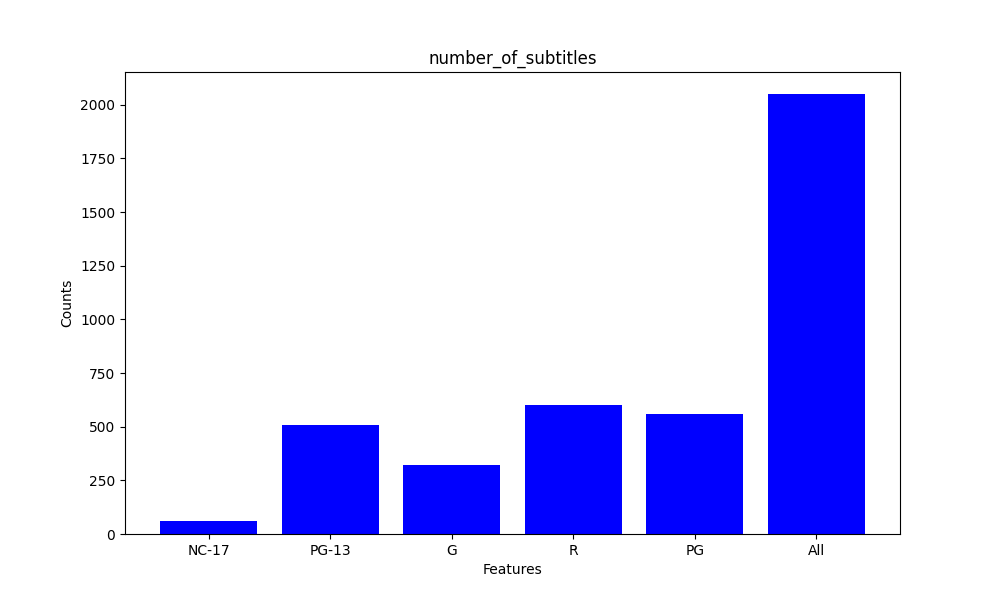
\includegraphics[width=1\textwidth]{../stats/number_of_subtitles.png}
    \caption{Number of subtitles}
\end{figure}

\begin{figure}[ht]
    \centering
    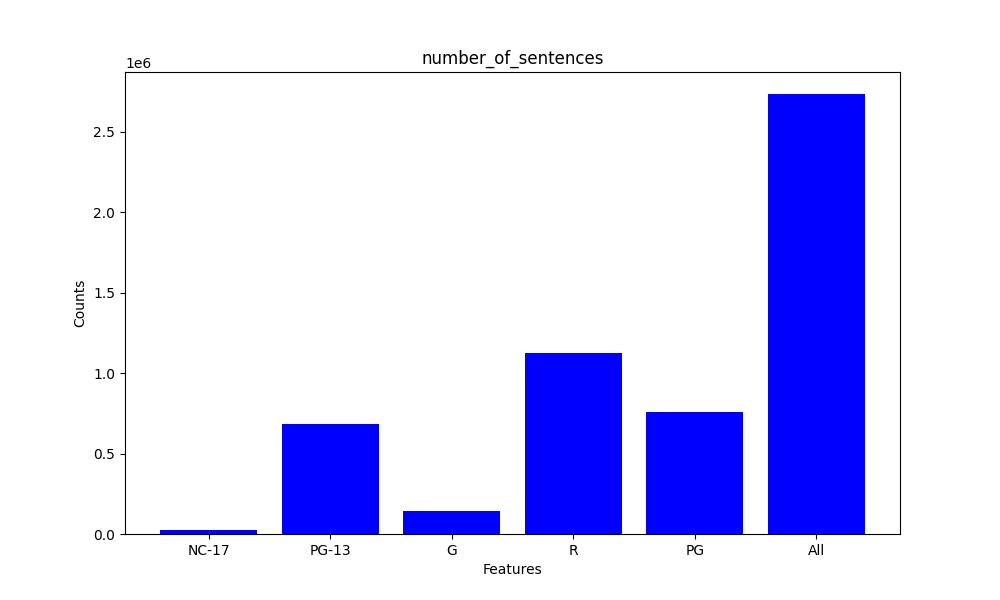
\includegraphics[width=1\textwidth]{../stats/number_of_sentences.png}
    \caption{Number of sentences}
\end{figure}

\begin{figure}[ht]
    \centering
    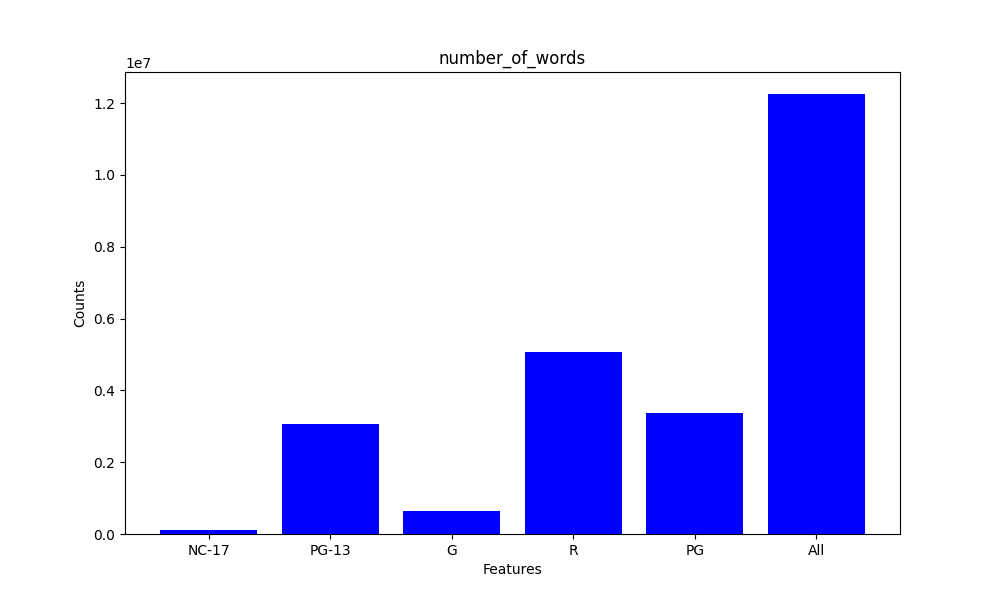
\includegraphics[width=1\textwidth]{../stats/number_of_words.png}
    \caption{Number of words}
\end{figure}

\begin{figure}[ht]
    \centering
    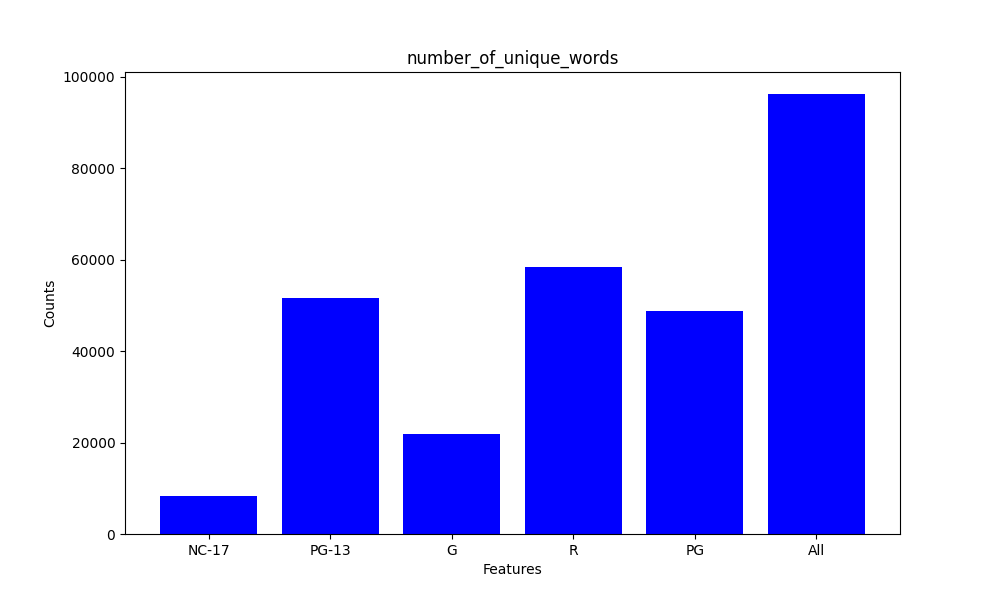
\includegraphics[width=1\textwidth]{../stats/number_of_unique_words.png}
    \caption{Number of unique words (non-duplicate)}
\end{figure}

\FloatBarrier

\subsection*{Number of unique words that are common and non-common in every two labels}

\begin{table}[ht]
    \centering
    \csvautotabular{../stats/commonTokens.csv}
    \caption{Common words}
    \label{tab:common_words}
\end{table}

\begin{table}[ht]
    \centering
    \csvautotabular{../stats/noncommonTokens.csv}

    \caption{Non-common words}
    \label{tab:non_common_words}
\end{table}

\FloatBarrier

\subsection*{Top words of each label based on frequency}

\begin{figure}[ht]
    \centering
    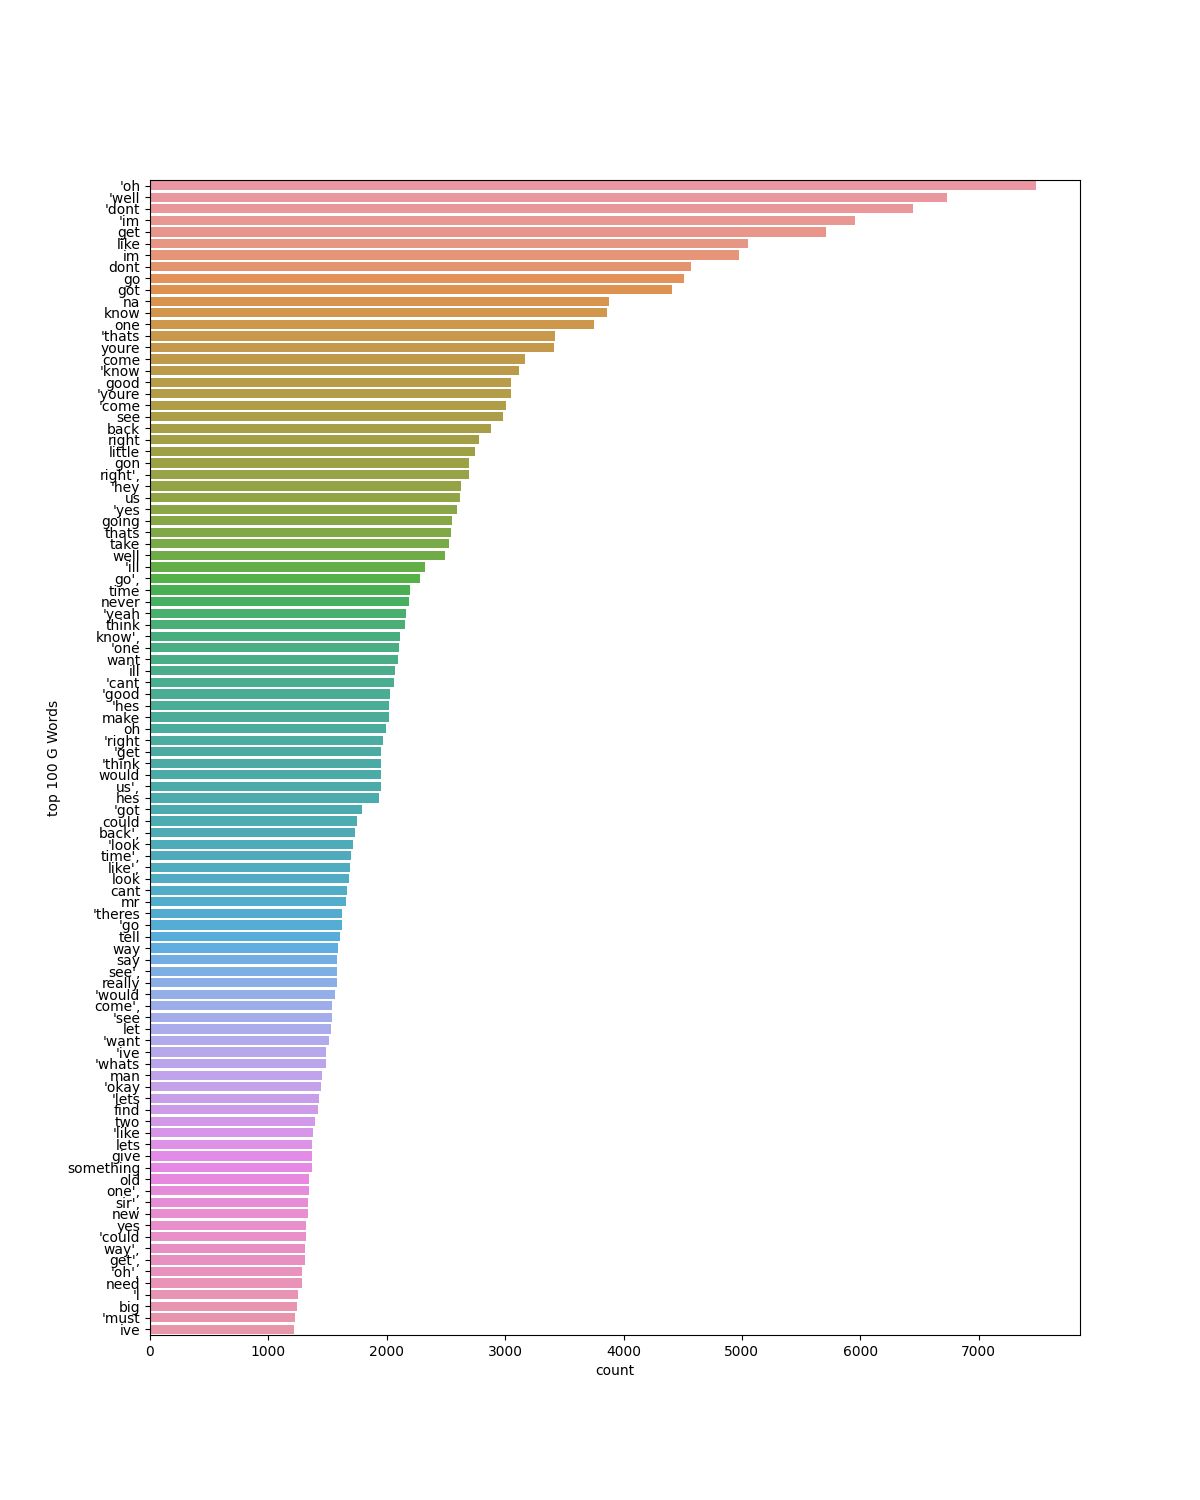
\includegraphics[width=1\textwidth]{../stats/top_100_G_words.png}
    \caption{Top 100 label G words}
\end{figure}

\begin{figure}[ht]
    \centering
    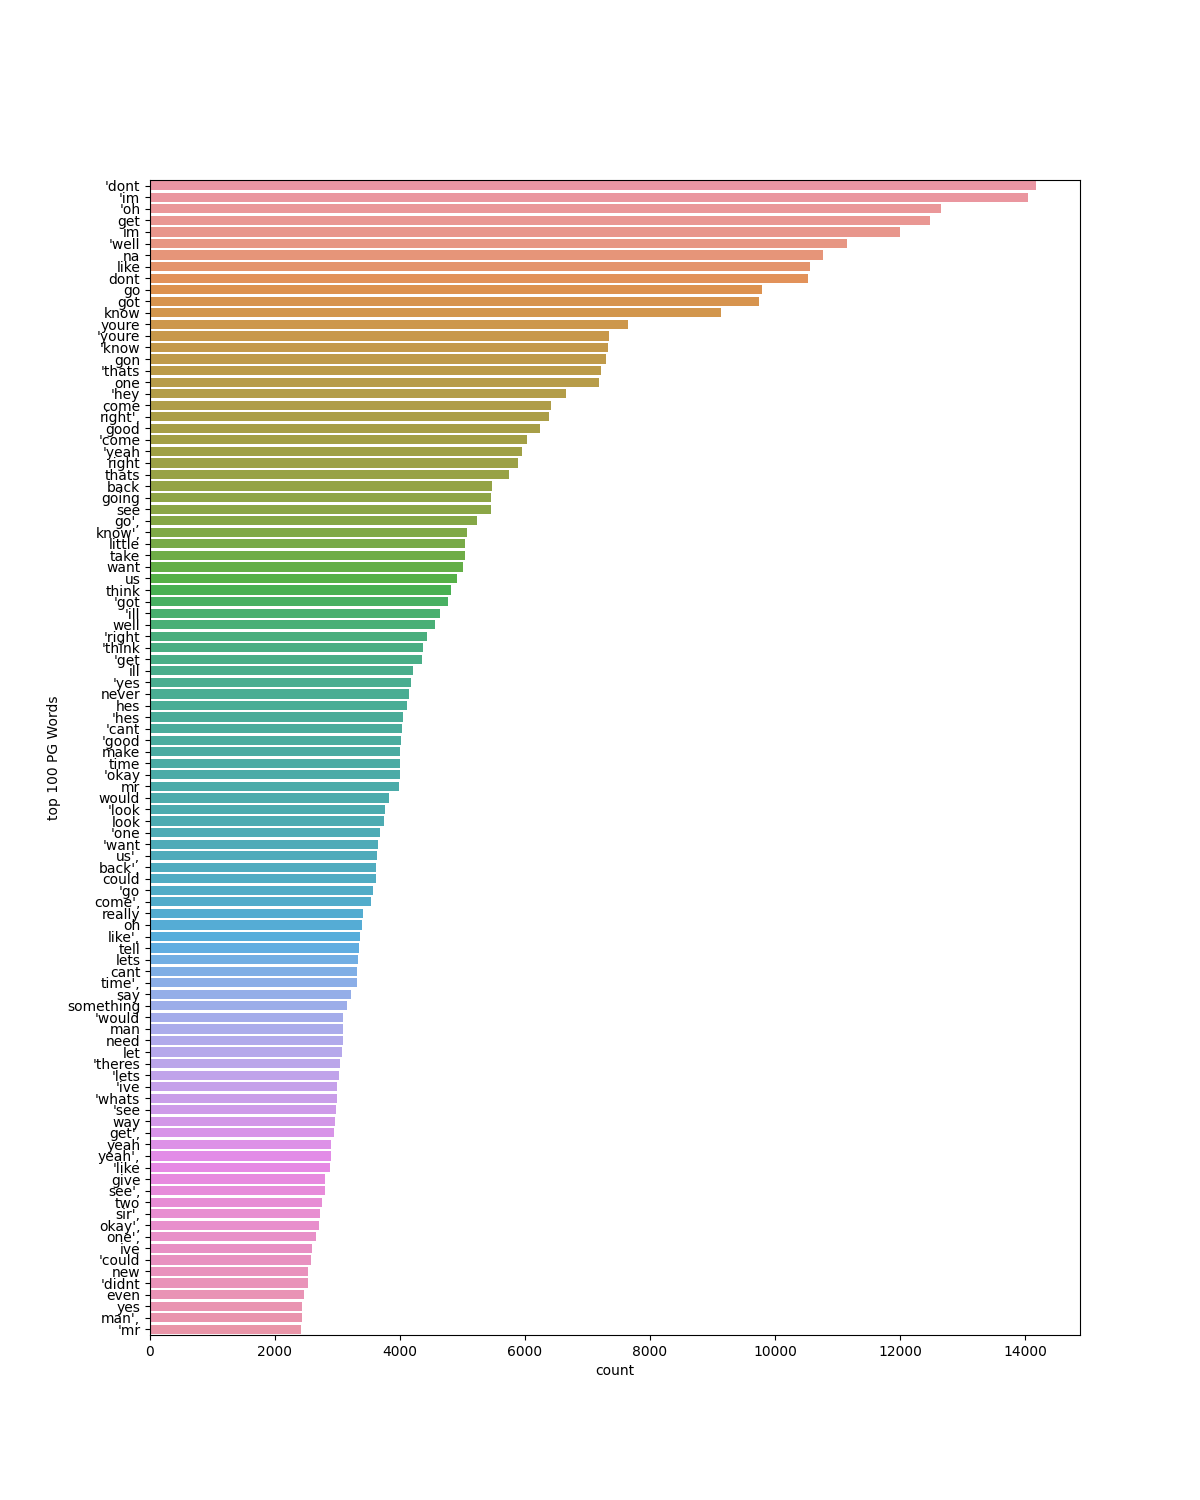
\includegraphics[width=1\textwidth]{../stats/top_100_PG_words.png}
    \caption{Top 100 label PG words}
\end{figure}

\begin{figure}[ht]
    \centering
    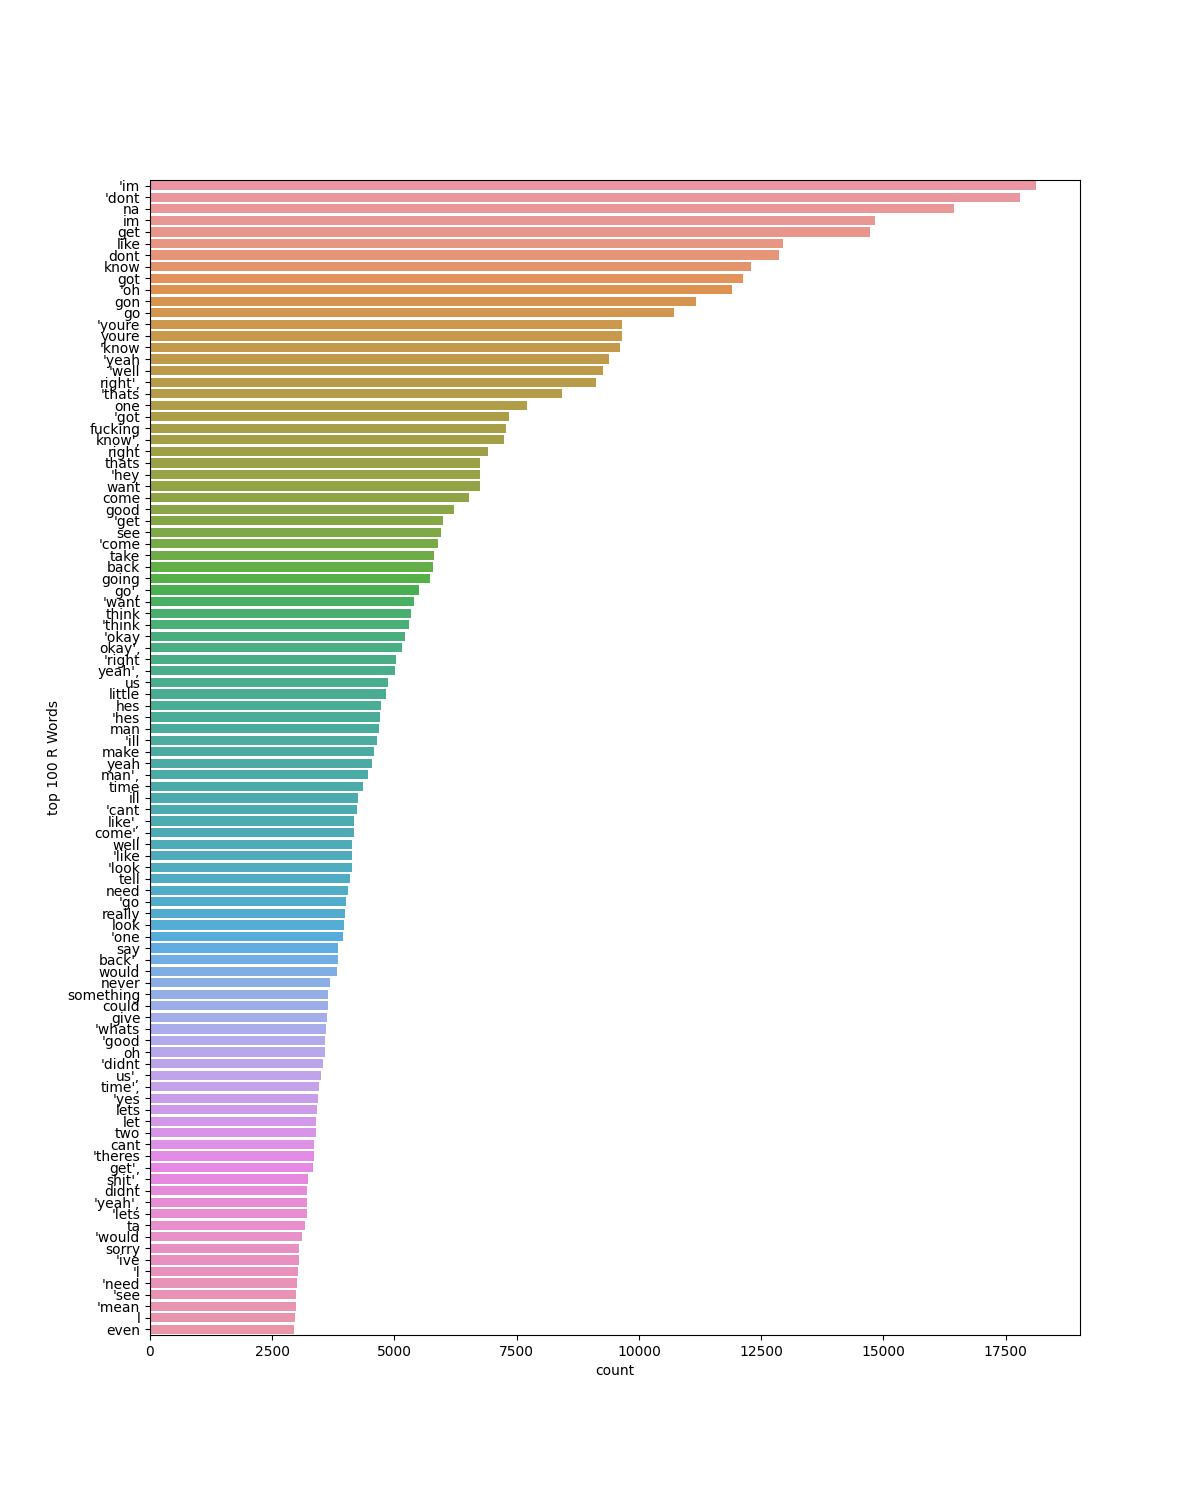
\includegraphics[width=1\textwidth]{../stats/top_100_R_words.png}
    \caption{Top 100 label R words}
\end{figure}

\begin{figure}[ht]
    \centering
    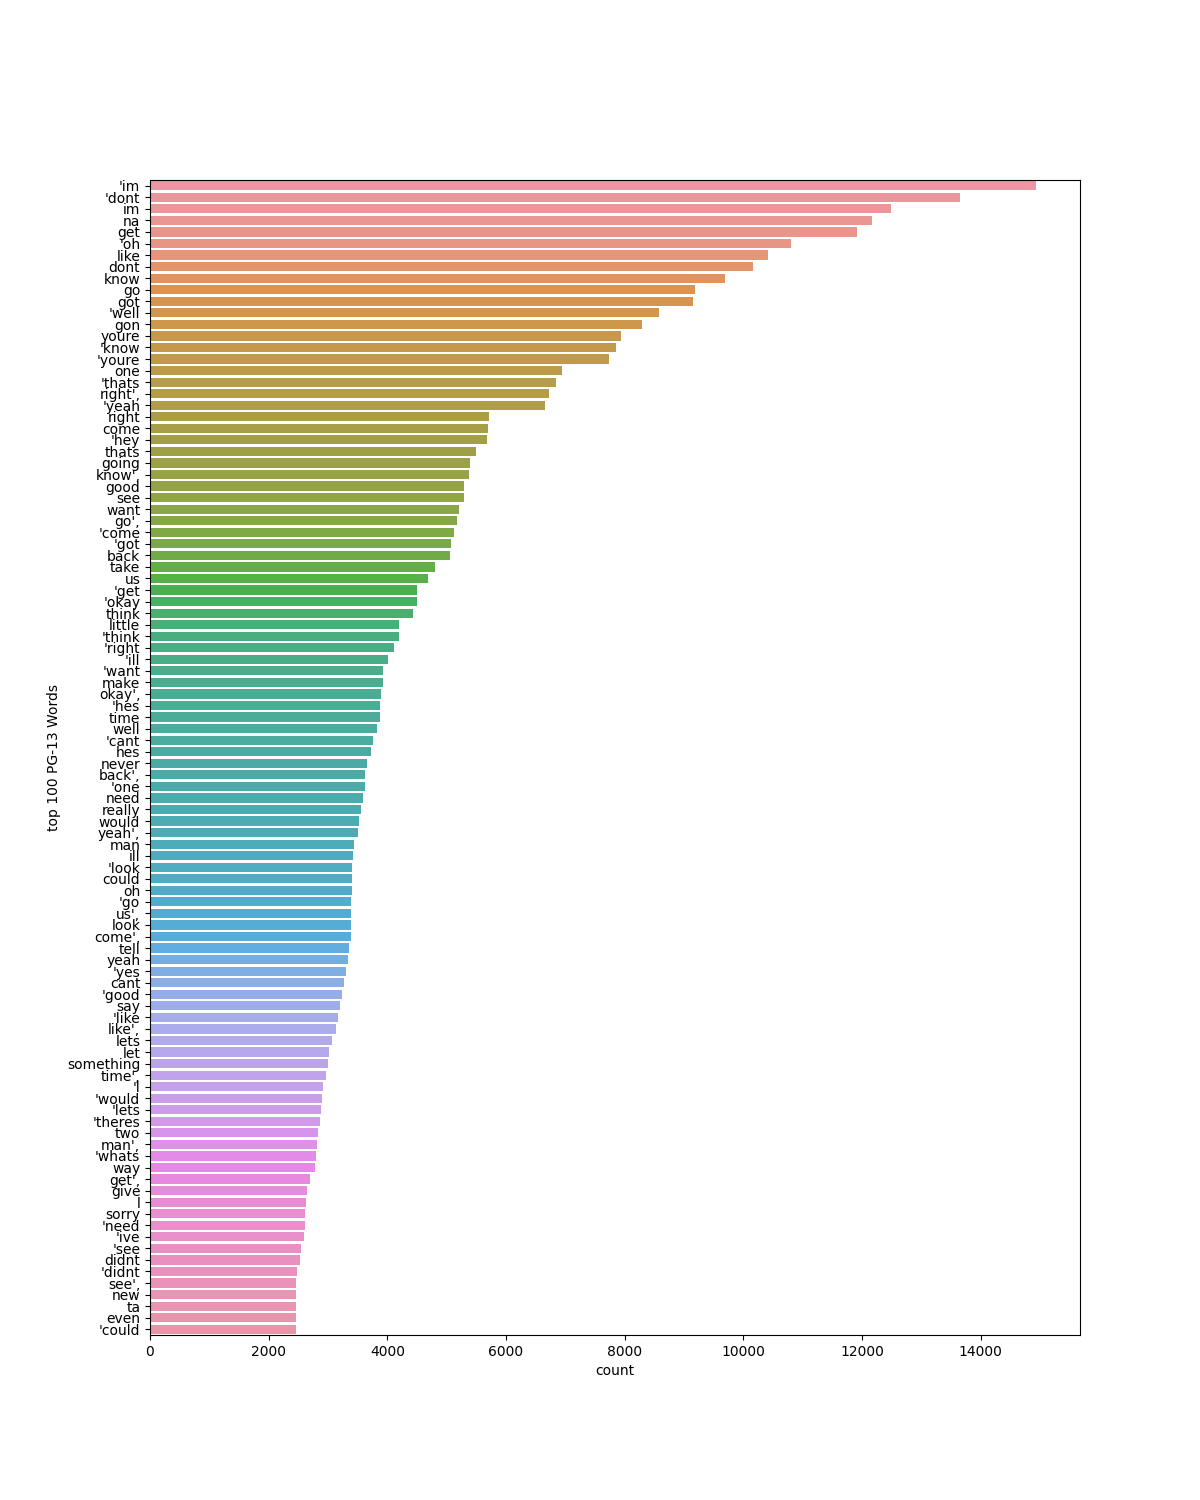
\includegraphics[width=1\textwidth]{../stats/top_100_PG-13_words.png}
    \caption{Top 100 label PG-13 words}
\end{figure}

\begin{figure}[ht]
    \centering
    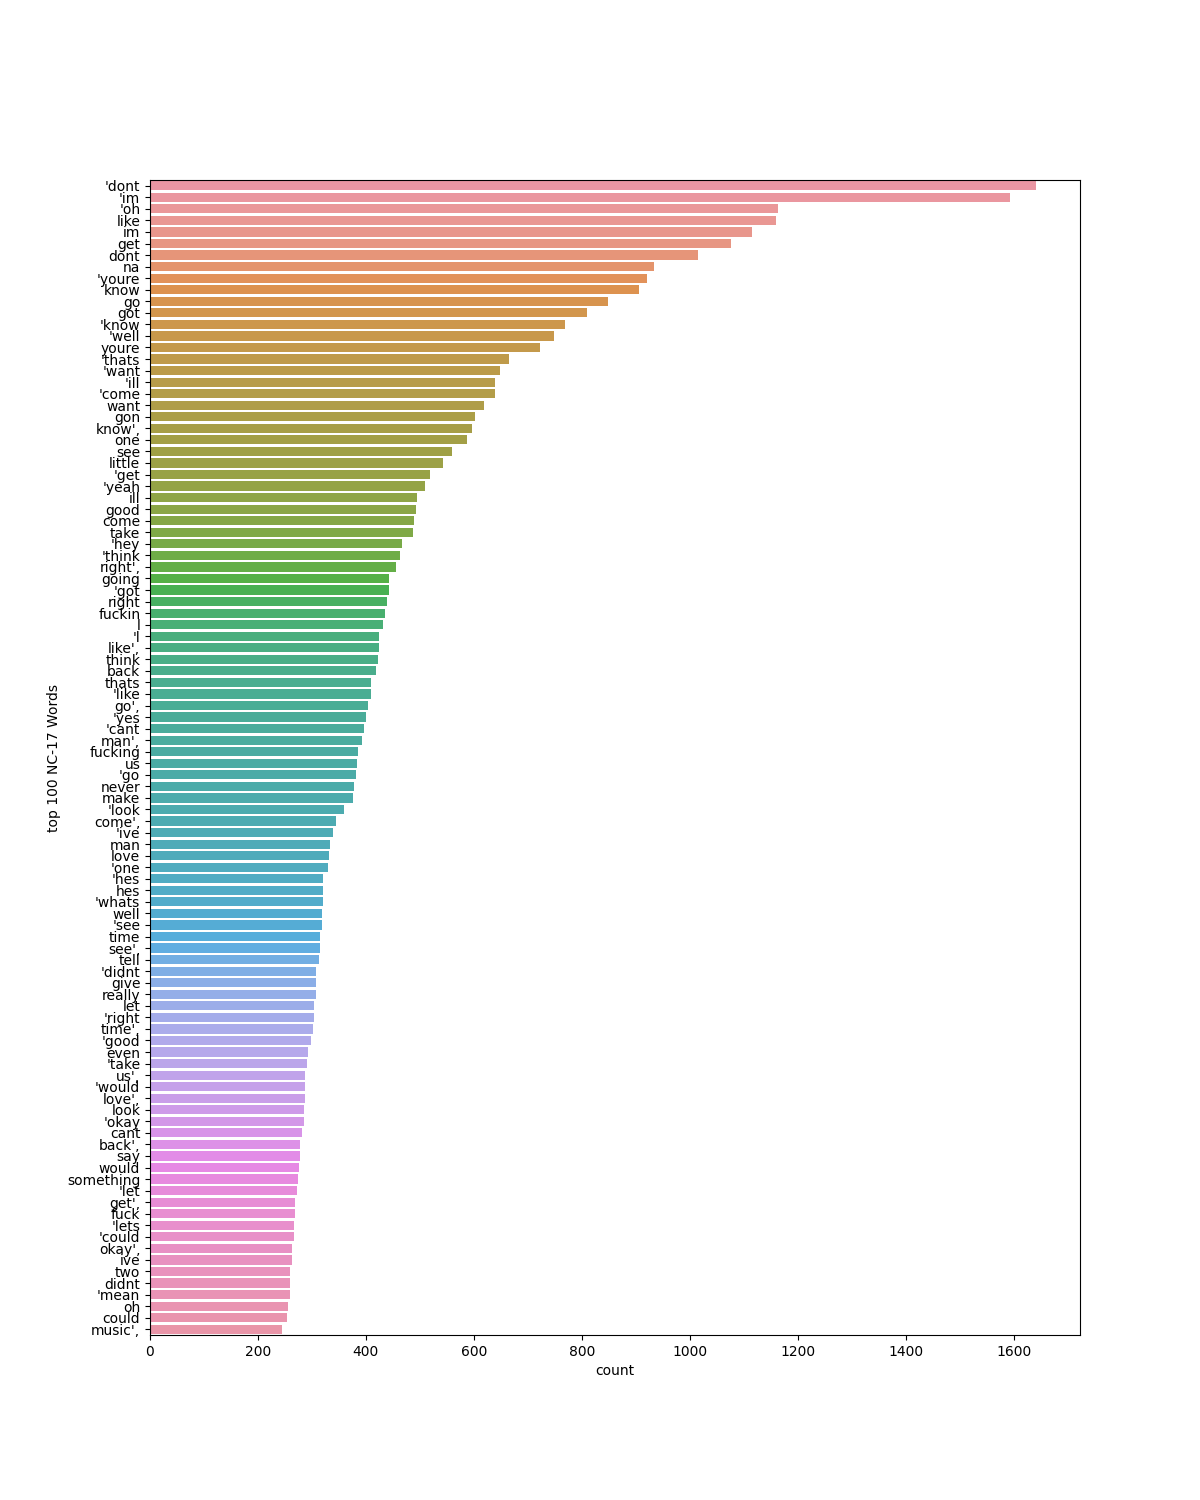
\includegraphics[width=1\textwidth]{../stats/top_100_NC-17_words.png}
    \caption{Top 100 label NC-17 words}
\end{figure}

\FloatBarrier

\subsection*{10 non-common words of each label}

\begin{figure}[ht]
    \centering
    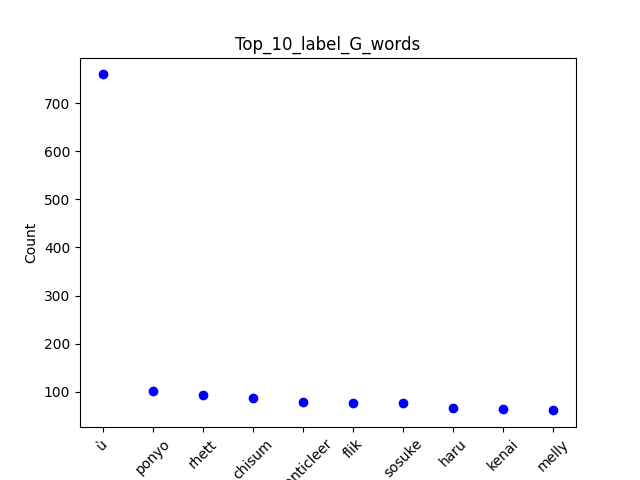
\includegraphics[width=1\textwidth]{../stats/Top_10_label_G_words.png}
    \caption{Top 10 label G words}
\end{figure}

\begin{figure}[ht]
    \centering
    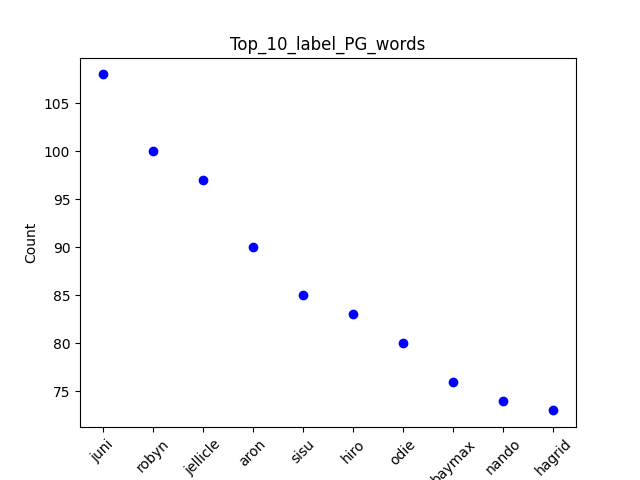
\includegraphics[width=1\textwidth]{../stats/Top_10_label_PG_words.png}
    \caption{Top 10 label PG words}
\end{figure}

\begin{figure}[ht]
    \centering
    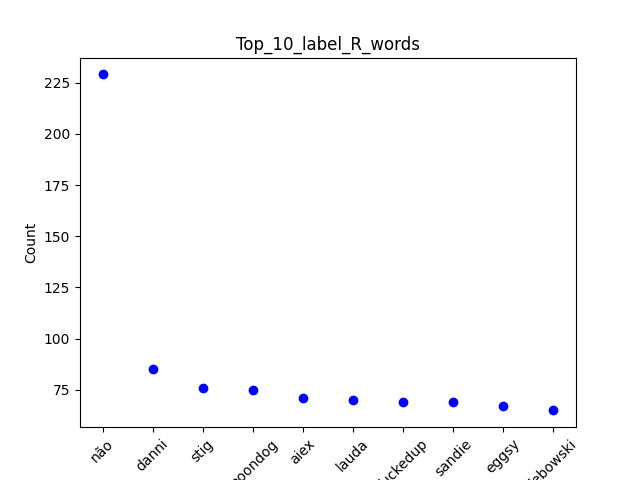
\includegraphics[width=1\textwidth]{../stats/Top_10_label_R_words.png}
    \caption{Top 10 label R words}
\end{figure}

\begin{figure}[ht]
    \centering
    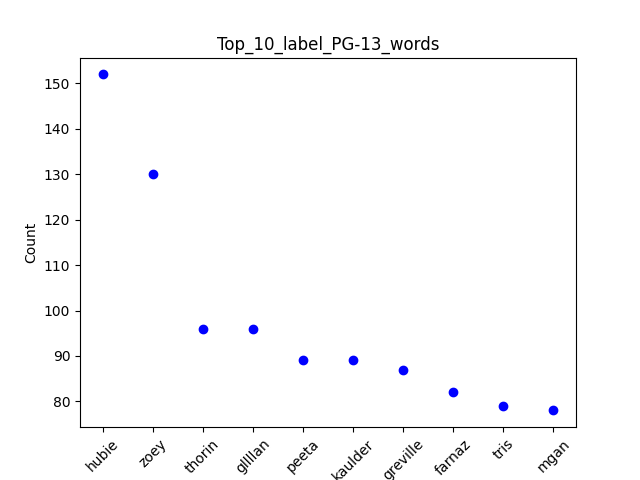
\includegraphics[width=1\textwidth]{../stats/Top_10_label_PG-13_words.png}
    \caption{Top 10 label PG-13 words}
\end{figure}

\begin{figure}[ht]
    \centering
    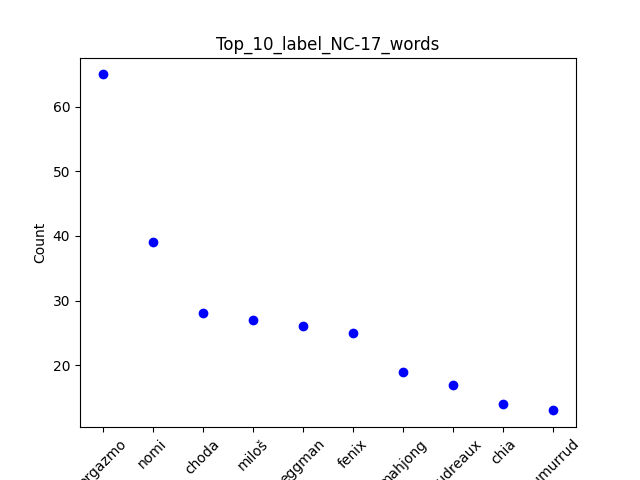
\includegraphics[width=1\textwidth]{../stats/Top_10_label_NC-17_words.png}
    \caption{Top 10 label NC-17 words}
\end{figure}

\FloatBarrier

\subsection*{The top 10 common words for each label compared to other labels based on the relative normalized frequency criterion.}

\begin{figure}[ht]
    \centering
    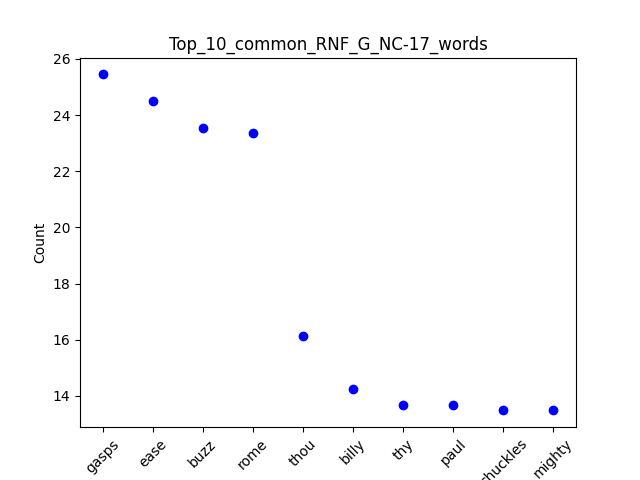
\includegraphics[width=1\textwidth]{../stats/Top_10_common_RNF_G_NC-17_words.png}
    \caption{RNF G NC-17}
\end{figure}


\begin{figure}[ht]
    \centering
    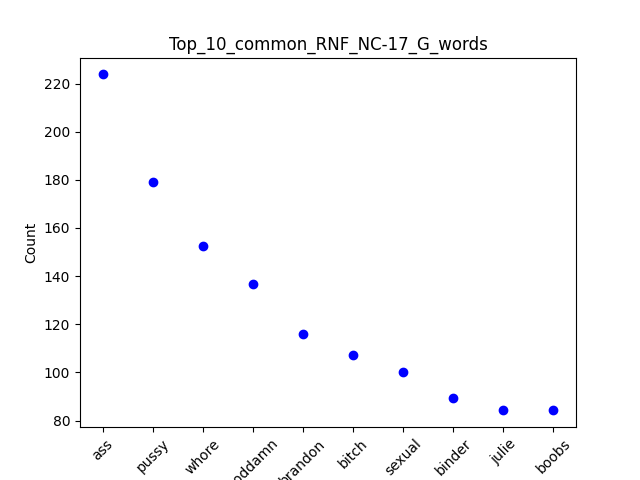
\includegraphics[width=1\textwidth]{../stats/Top_10_common_RNF_NC-17_G_words.png}
    \caption{RNF NC-17 G}
\end{figure}


\begin{figure}[ht]
    \centering
    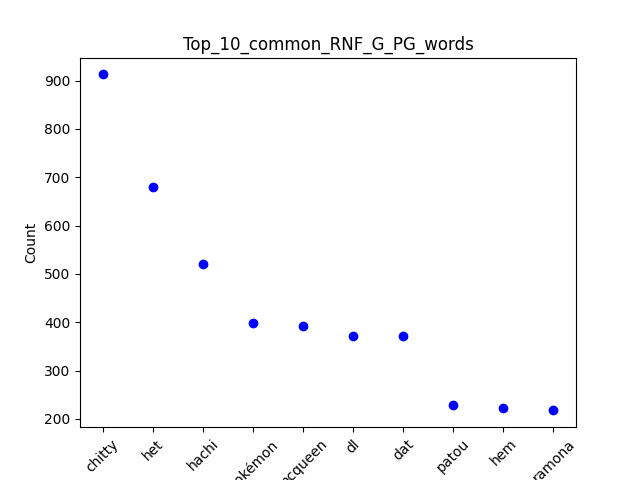
\includegraphics[width=1\textwidth]{../stats/Top_10_common_RNF_G_PG_words.png}
    \caption{RNF G PG}
\end{figure}


\begin{figure}[ht]
    \centering
    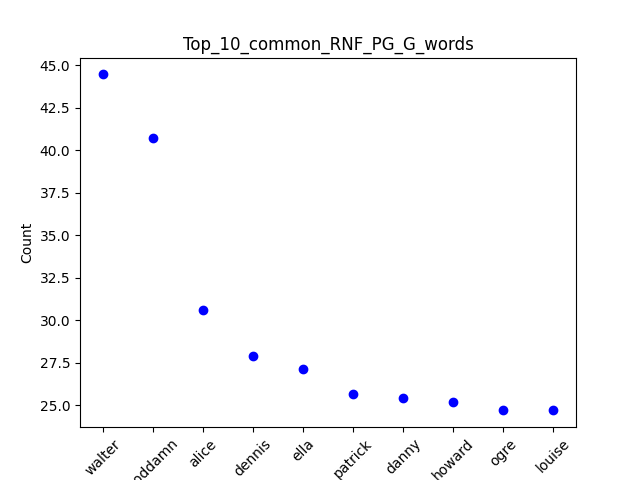
\includegraphics[width=1\textwidth]{../stats/Top_10_common_RNF_PG_G_words.png}
    \caption{RNF PG G}
\end{figure}


\begin{figure}[ht]
    \centering
    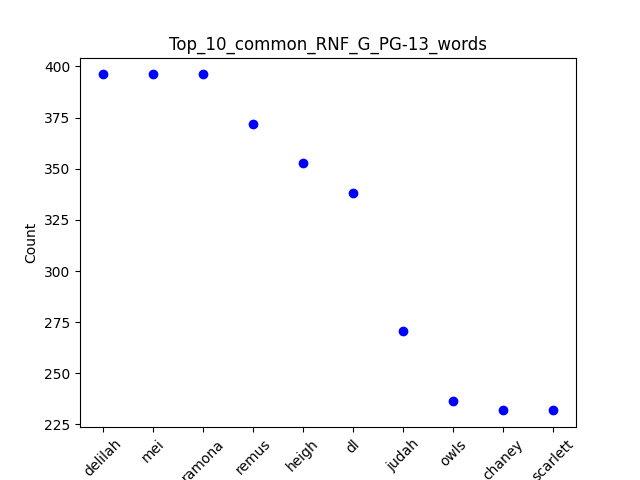
\includegraphics[width=1\textwidth]{../stats/Top_10_common_RNF_G_PG-13_words.png}
    \caption{RNF G PG-13}
\end{figure}


\begin{figure}[ht]
    \centering
    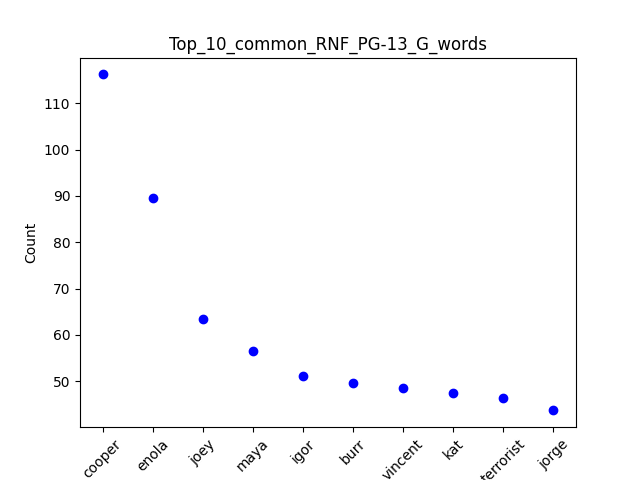
\includegraphics[width=1\textwidth]{../stats/Top_10_common_RNF_PG-13_G_words.png}
    \caption{RNF PG-13 G}
\end{figure}


\begin{figure}[ht]
    \centering
    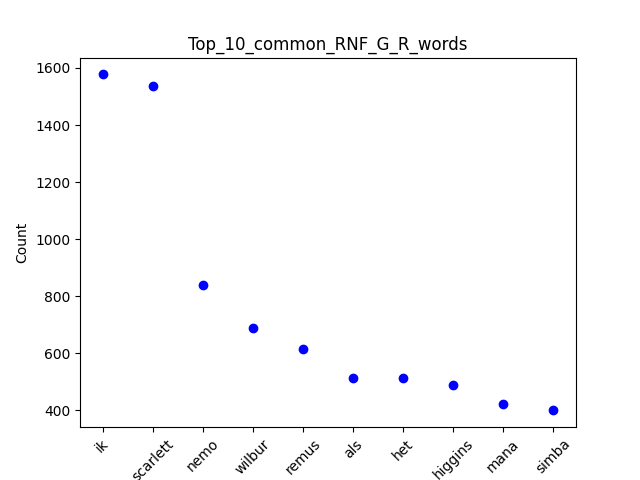
\includegraphics[width=1\textwidth]{../stats/Top_10_common_RNF_G_R_words.png}
    \caption{RNF G R}
\end{figure}


\begin{figure}[ht]
    \centering
    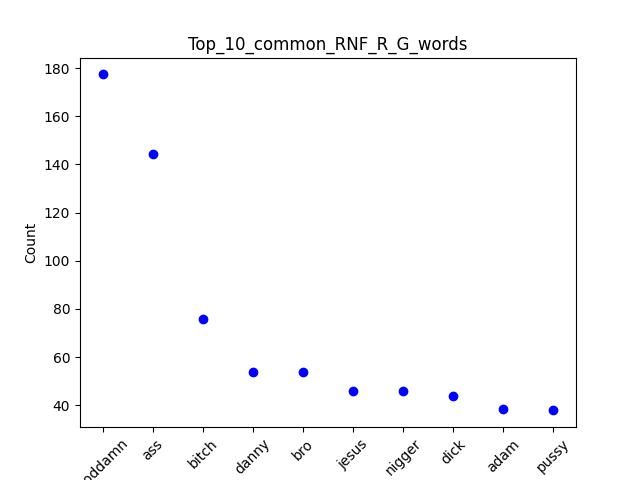
\includegraphics[width=1\textwidth]{../stats/Top_10_common_RNF_R_G_words.png}
    \caption{RNF R G}
\end{figure}


\begin{figure}[ht]
    \centering
    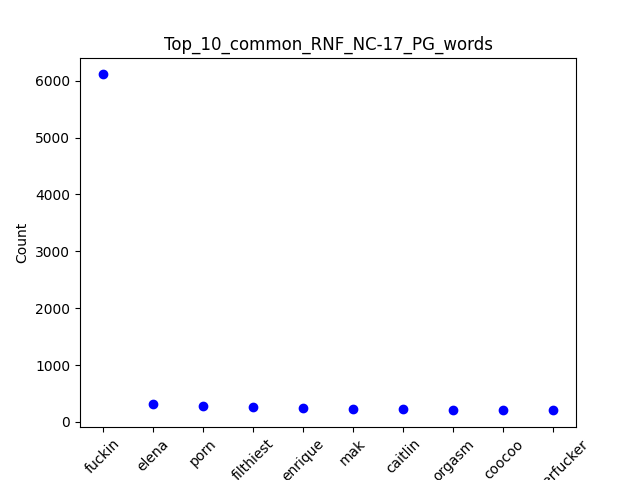
\includegraphics[width=1\textwidth]{../stats/Top_10_common_RNF_NC-17_PG_words.png}
    \caption{RNF NC-17 PG}
\end{figure}


\begin{figure}[ht]
    \centering
    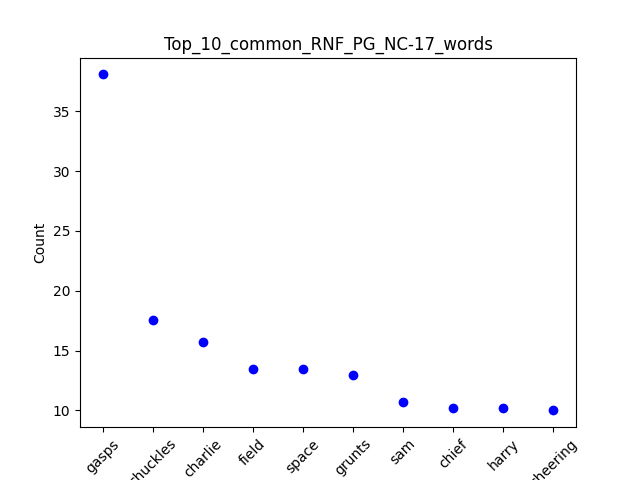
\includegraphics[width=1\textwidth]{../stats/Top_10_common_RNF_PG_NC-17_words.png}
    \caption{RNF PG NC-17}
\end{figure}


\begin{figure}[ht]
    \centering
    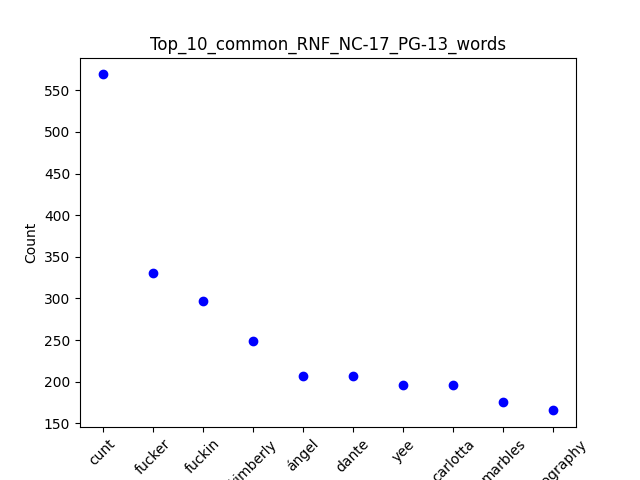
\includegraphics[width=1\textwidth]{../stats/Top_10_common_RNF_NC-17_PG-13_words.png}
    \caption{RNF NC-17 PG-13}
\end{figure}


\begin{figure}[ht]
    \centering
    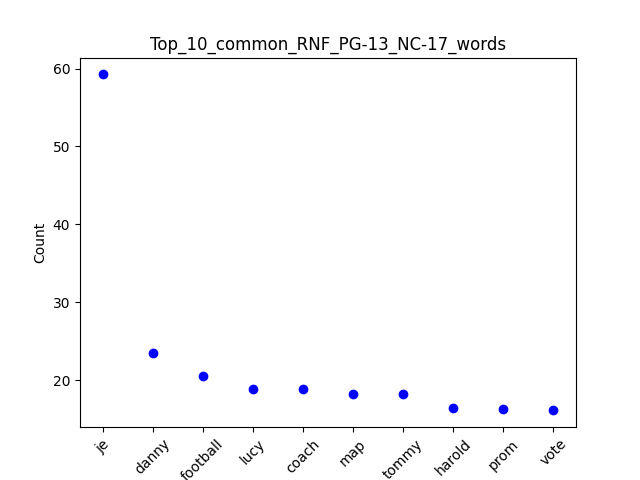
\includegraphics[width=1\textwidth]{../stats/Top_10_common_RNF_PG-13_NC-17_words.png}
    \caption{RNF PG-13 NC-17}
\end{figure}


\begin{figure}[ht]
    \centering
    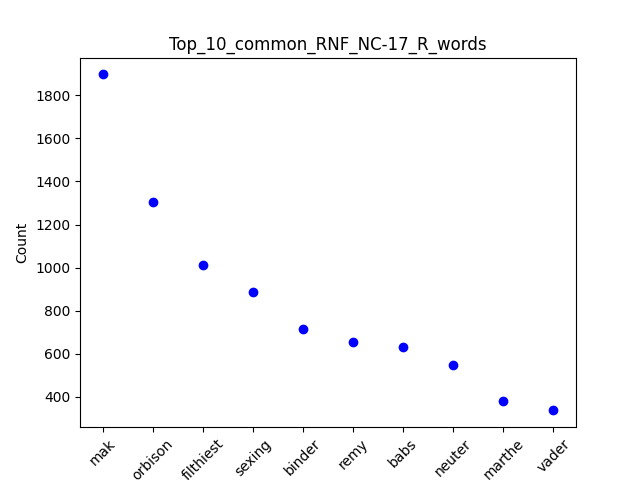
\includegraphics[width=1\textwidth]{../stats/Top_10_common_RNF_NC-17_R_words.png}
    \caption{RNF NC-17 R}
\end{figure}


\begin{figure}[ht]
    \centering
    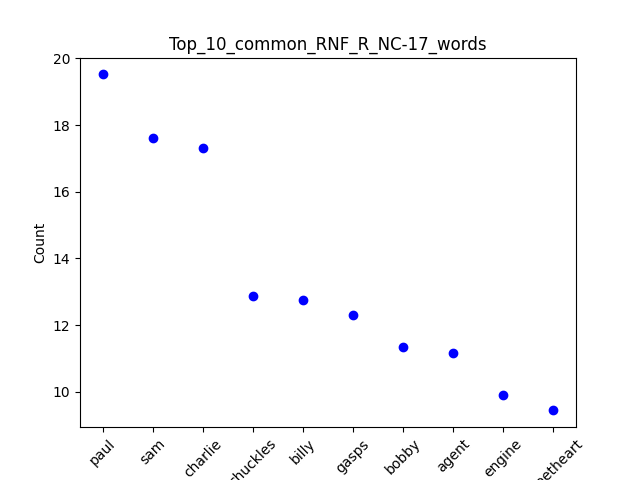
\includegraphics[width=1\textwidth]{../stats/Top_10_common_RNF_R_NC-17_words.png}
    \caption{RNF R NC-17}
\end{figure}


\begin{figure}[ht]
    \centering
    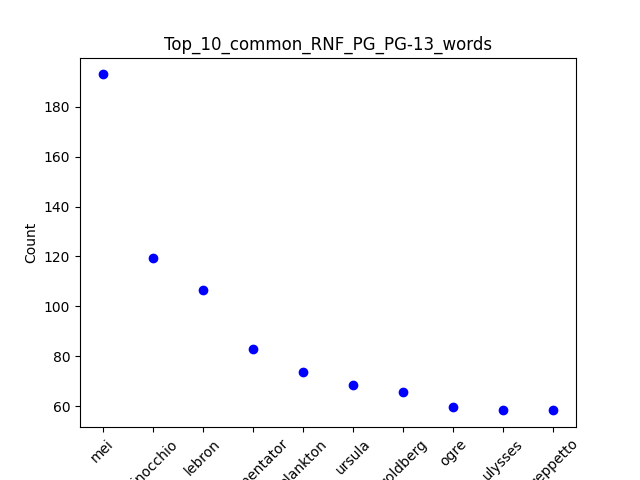
\includegraphics[width=1\textwidth]{../stats/Top_10_common_RNF_PG_PG-13_words.png}
    \caption{RNF PG PG-13}
\end{figure}


\begin{figure}[ht]
    \centering
    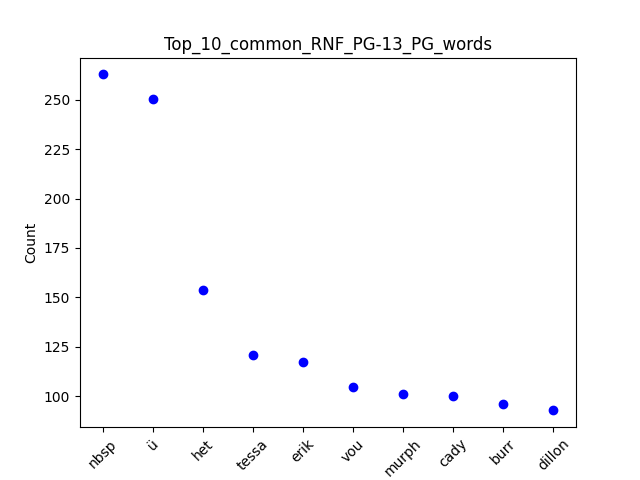
\includegraphics[width=1\textwidth]{../stats/Top_10_common_RNF_PG-13_PG_words.png}
    \caption{RNF PG-13 PG}
\end{figure}


\begin{figure}[ht]
    \centering
    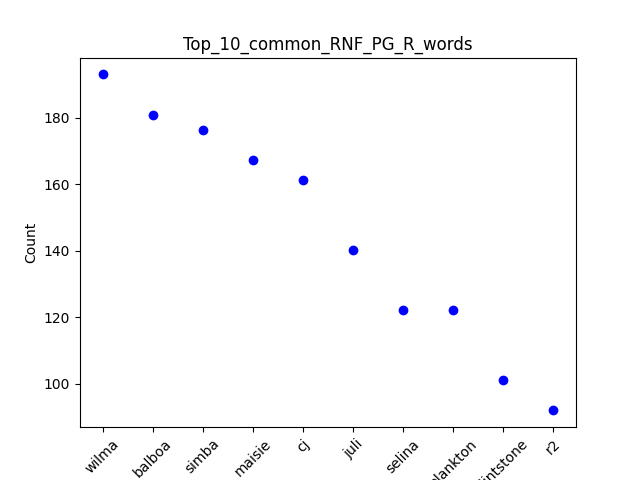
\includegraphics[width=1\textwidth]{../stats/Top_10_common_RNF_PG_R_words.png}
    \caption{RNF PG R}
\end{figure}


\begin{figure}[ht]
    \centering
    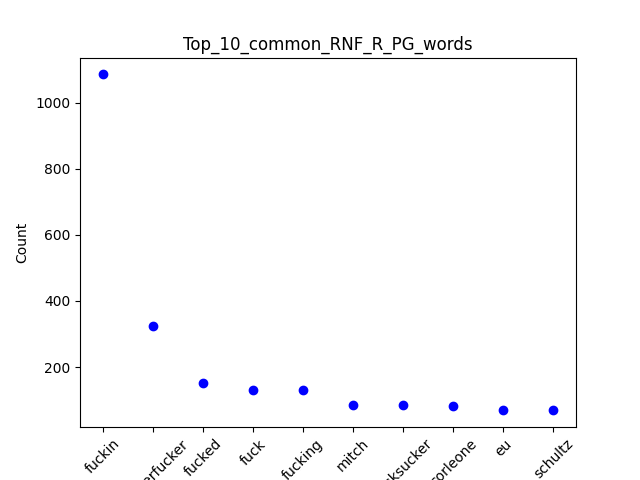
\includegraphics[width=1\textwidth]{../stats/Top_10_common_RNF_R_PG_words.png}
    \caption{RNF R PG}
\end{figure}


\begin{figure}[ht]
    \centering
    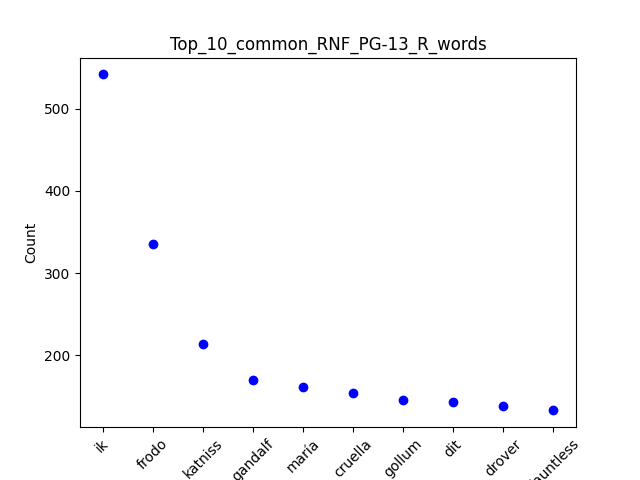
\includegraphics[width=1\textwidth]{../stats/Top_10_common_RNF_PG-13_R_words.png}
    \caption{RNF PG-13 R}
\end{figure}


\begin{figure}[ht]
    \centering
    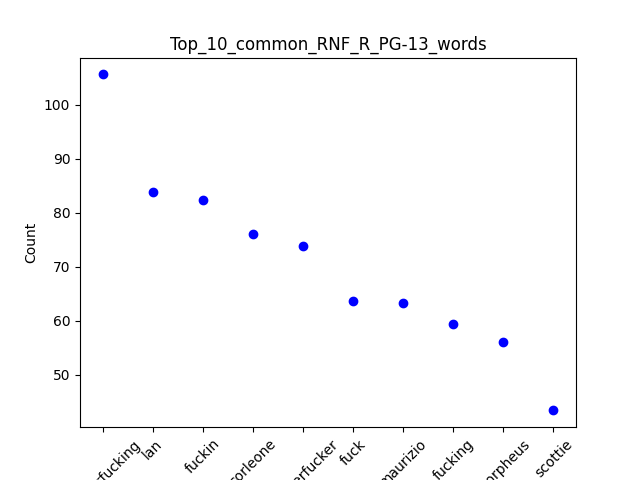
\includegraphics[width=1\textwidth]{../stats/Top_10_common_RNF_R_PG-13_words.png}
    \caption{RNF R PG-13}
\end{figure}


\FloatBarrier

\subsection*{Top 10 Words for each label based of TF-IDF}

\begin{figure}[ht]
    \centering
    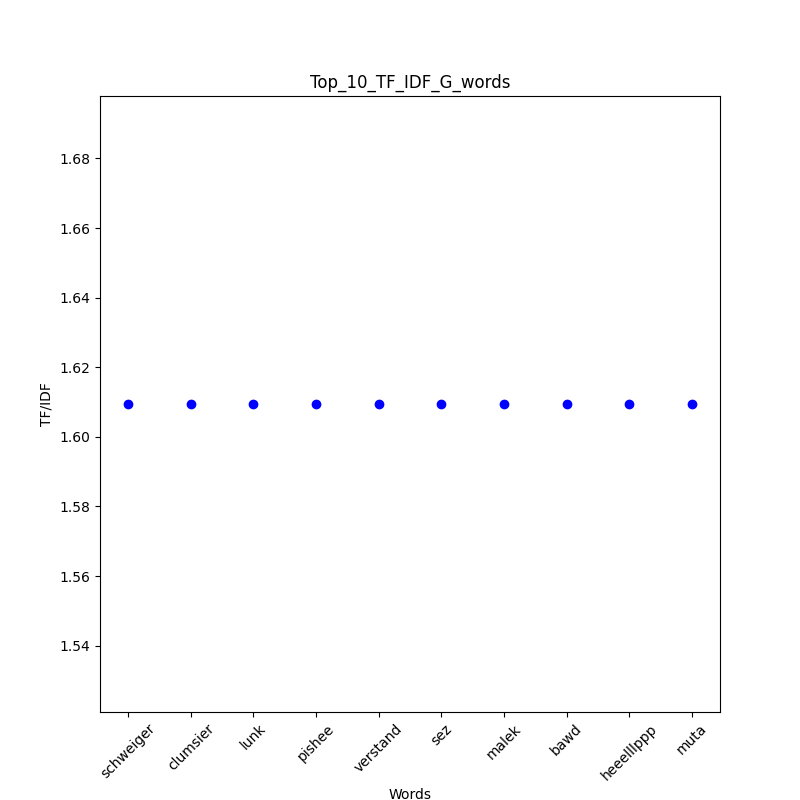
\includegraphics[width=1\textwidth]{../stats/Top_10_TF_IDF_G_words.png}
    \caption{Top 10 TF-IDF G words}
\end{figure}

\begin{figure}[ht]
    \centering
    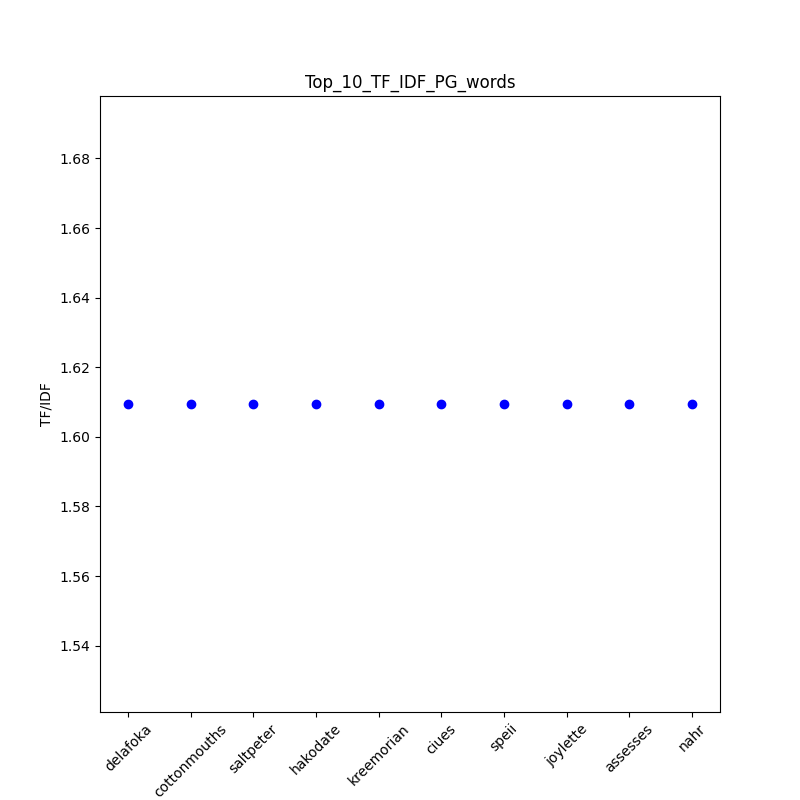
\includegraphics[width=1\textwidth]{../stats/Top_10_TF_IDF_PG_words.png}
    \caption{Top 10 TF-IDF PG words}
\end{figure}

\begin{figure}[ht]
    \centering
    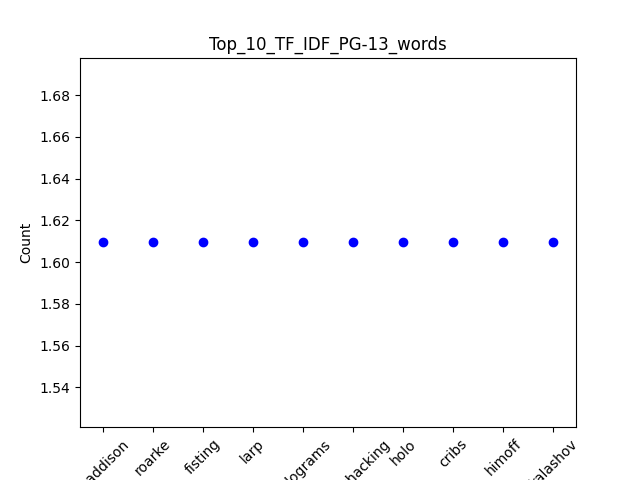
\includegraphics[width=1\textwidth]{../stats/Top_10_TF_IDF_PG-13_words.png}
    \caption{Top 10 TF-IDF PG-13 words}
\end{figure}

\begin{figure}[ht]
    \centering
    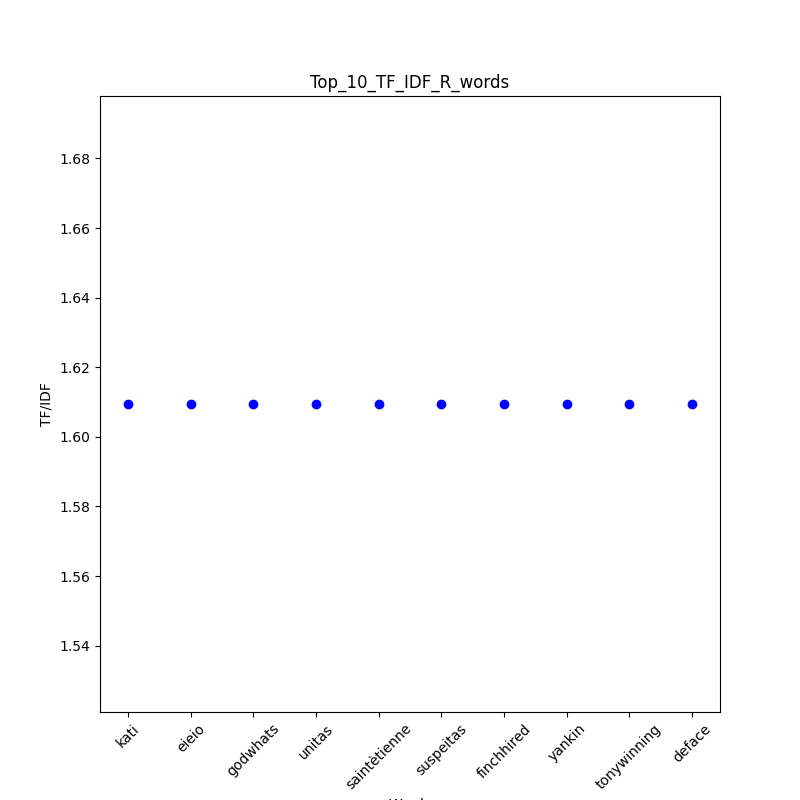
\includegraphics[width=1\textwidth]{../stats/Top_10_TF_IDF_R_words.png}
    \caption{Top 10 TF-IDF R words}
\end{figure}

\begin{figure}[ht]
    \centering
    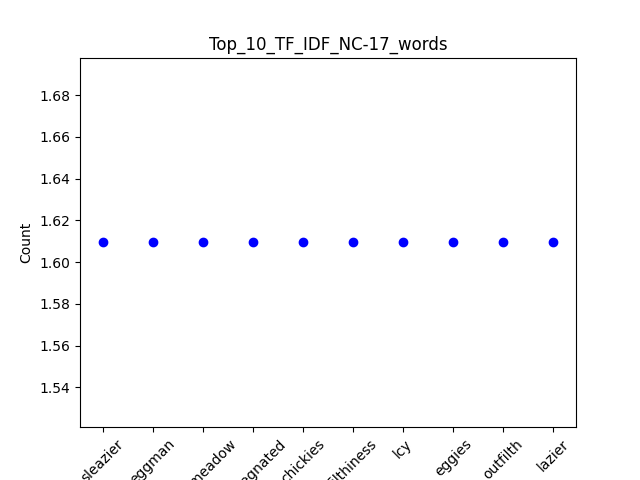
\includegraphics[width=1\textwidth]{../stats/Top_10_TF_IDF_NC-17_words.png}
    \caption{Top 10 TF-IDF NC-17 words}
\end{figure}

\FloatBarrier

\subsection*{Top 15 Words for each label histogram ( from high to low freq )}

\begin{figure}[ht]
    \centering
    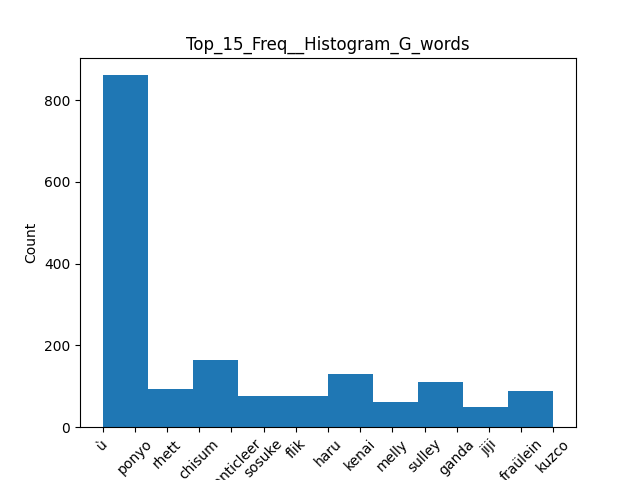
\includegraphics[width=1\textwidth]{../stats/Top_15_Freq__Histogram_G_Words.png}
    \caption{Top 15 Freq Histogram G Words}
\end{figure}

\begin{figure}[ht]
    \centering
    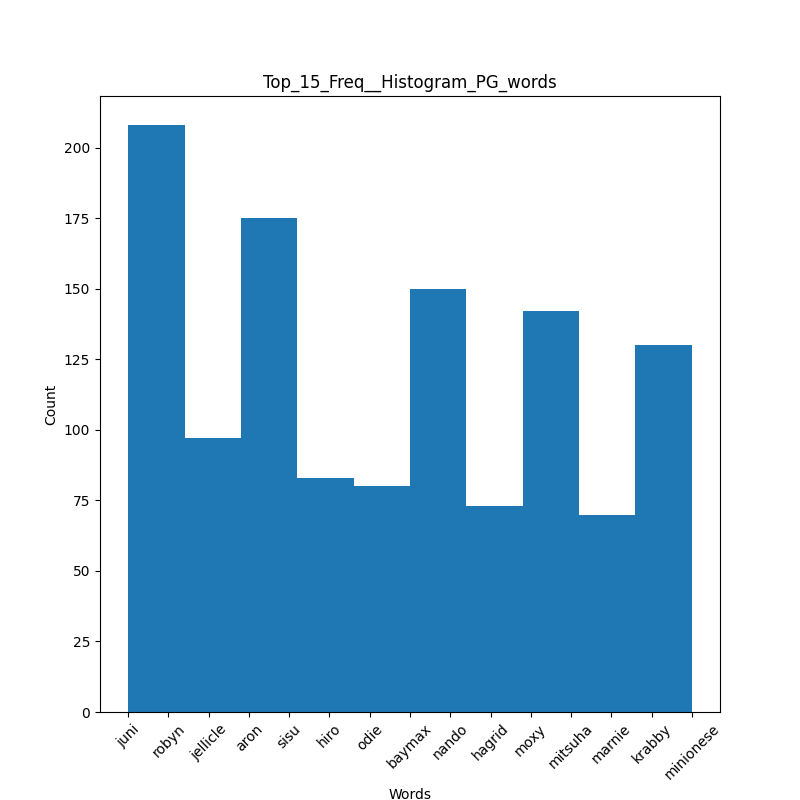
\includegraphics[width=1\textwidth]{../stats/Top_15_Freq__Histogram_PG_Words.png}
    \caption{Top 15 Freq Histogram PG Words}
\end{figure}

\begin{figure}[ht]
    \centering
    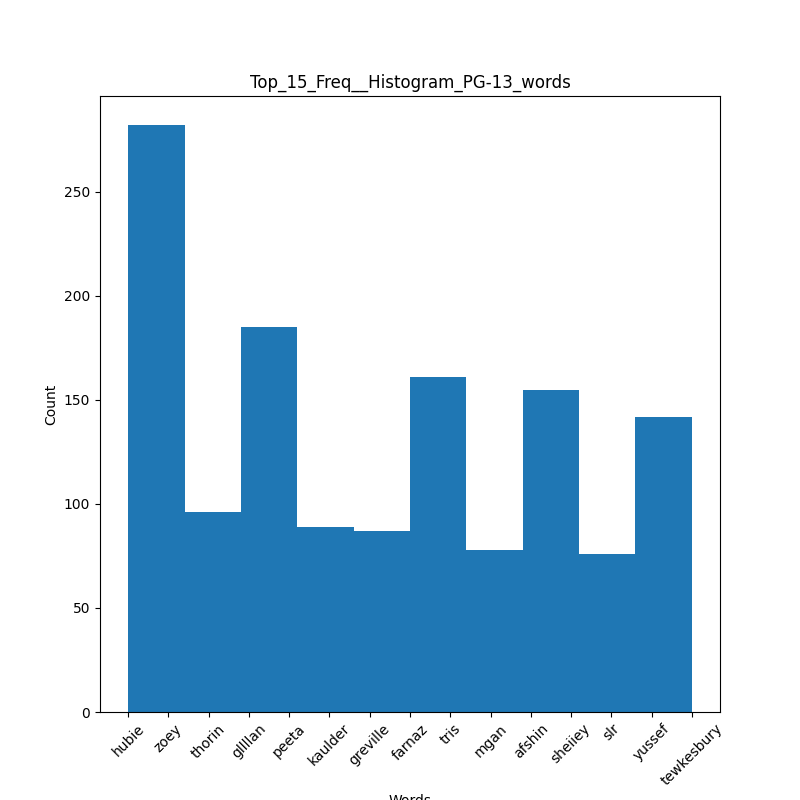
\includegraphics[width=1\textwidth]{../stats/Top_15_Freq__Histogram_PG-13_Words.png}
    \caption{Top 15 Freq Histogram PG-13 Words}
\end{figure}

\begin{figure}[ht]
    \centering
    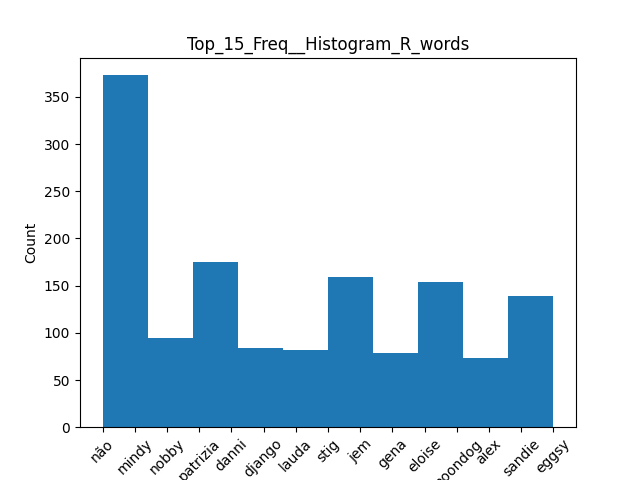
\includegraphics[width=1\textwidth]{../stats/Top_15_Freq__Histogram_R_Words.png}
    \caption{Top 15 Freq Histogram R Words}
\end{figure}

\begin{figure}[ht]
    \centering
    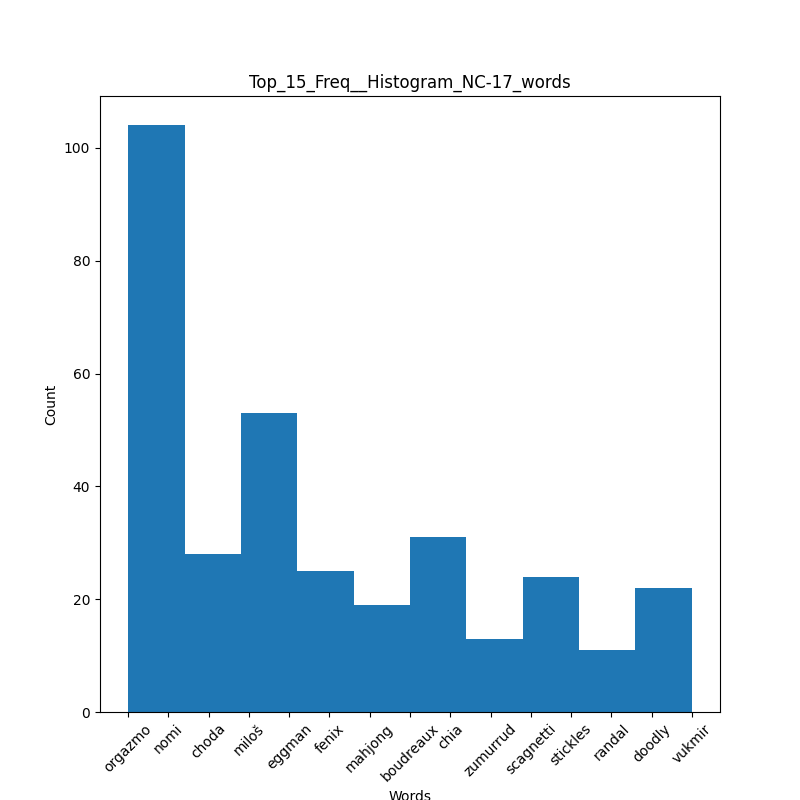
\includegraphics[width=1\textwidth]{../stats/Top_15_Freq__Histogram_NC-17_Words.png}
    \caption{Top 15 Freq Histogram NC-17 Words}
\end{figure}

\end{document}